\documentclass[a4paper,12pt,oneside,openany,table,xcdraw]{article}

\usepackage{setspace}
\usepackage{multirow}
\usepackage{hyperref}
\usepackage{caption}
\usepackage{indentfirst}
\usepackage{tikz} %% fasores
\usetikzlibrary{arrows,arrows.meta,quotes,angles}
\usepackage{siunitx}

\usepackage[brazilian]{babel}
\usepackage[utf8x]{inputenc}
\usepackage{amsmath, graphicx, subfig, enumerate}
\usepackage{float, verbatim}
\usepackage[colorinlistoftodos]{todonotes}
\usepackage{makeidx}
\usepackage{geometry}

\graphicspath{{img/}}
\geometry{a4paper, hmargin={3cm, 3cm}, vmargin={3cm, 2cm} }
\setlength{\parindent}{1.0cm}
\captionsetup{font=small}

\begin{document}
\newcommand{\thedepartment}{Faculdade de Engenharia Elétrica}
\newcommand{\thecourse}{FEELT}
\newcommand{\thetitle}{ANÁLISE DE ONDAS NÃO SENOIDAIS - LÂMPADAS (CARGAS NÃO LINEARES)}
\newcommand{\thetype}{Relatório da Disciplina de Experimental de Circuitos Elétricos II}
\newcommand{\theproftitle}{Bacharel em Engenharia Elétrica}
\newcommand{\thestudent}{Lesly Viviane Montúfar Berrios\\
\centering11811ETE001}
\newcommand{\theadvisor}{Prof. Wellington Maycon Santos Bernardes}
\newcommand{\thecity}{Uberlândia}

\thispagestyle{empty}\newcommand*{\themonth}{\ifthenelse{\the\month < 2}{Janeiro }
                  {\ifthenelse{\the\month < 3}{Fevereiro }
                  {\ifthenelse{\the\month < 4}{Março }
                  {\ifthenelse{\the\month < 5}{Abril }
                  {\ifthenelse{\the\month < 6}{Maio }
                  {\ifthenelse{\the\month < 7}{Junho }
                  {\ifthenelse{\the\month < 8}{Julho }
                  {\ifthenelse{\the\month < 9}{Agosto }
                  {\ifthenelse{\the\month < 10}{Setembro }
                  {\ifthenelse{\the\month < 11}{Outubro }
                  {\ifthenelse{\the\month < 12}{Novembro }{Dezembro }}}}}}}}}}}}
                  
\begin{titlepage}
\begin{center}

	\vspace{-0.5cm}

  \begin{figure}[hbt!]
		\begin{center}
		   
\includegraphics[width=2.8cm]{ufu-logo.png}
		\end{center}
	\end{figure}
 	%\vspace{-4cm}

%\begin{doublespacing}

  \Large{\textbf{Universidade Federal de Uberlândia}}\\
  \large{\thedepartment}\\
  \large{\thecourse}\\


\vspace{5.8cm}
  \par
  \large\textbf{\thetitle}
\vspace{5.8cm} 

%\end{doublespacing}
  \par
  \thetype\\
  por\\
  %\hspace{2cm}\large{}\\

\vspace{0.8cm}
\par
  \normalsize{\thestudent}\\ [2cm]
  \theadvisor

\par\vfill
  \thecity, \themonth / \the\year

\end{center}

\end{titlepage}

%% Comeca o documento !

\onehalfspacing
\tableofcontents % sumário
\newpage

\section{Objetivos} % 2,5%
Pretende-se verificar experimentalmente conceitos teóricos de sinais não senoidais, obtendo os coeficientes da série de Fourier pelo método analítico e usando uma rotina computacional (como Matlab, Python). Aqui também é investigada a determinação do valor eficazes (rms) da tensão e corrente, bem como as potências associadas das formas de onda não senoidais.

\section{Introdução teórica} % 5%

Ondas não senoidais na rede são bastante comuns e surgem da presença de cargas não-lineares na rede (proporção tensão e corrente não é constante). Alguns exemplos de cargas geradoras de correntes harmônicas são geradores e motores CA, transformadores, lâmpadas de descarga, retificadores/motores CC controlados, inversores/motores de indução, ciclo-conversores/motores síncronos, cargas de aquecimento controladas por tiristores, reguladores de tensão a núcleo saturado, computadores etc \cite{PH}. 

Na Figura \ref{intro:fig1} observa-se uma característica importante para ondas com distorção harmônica. A corrente fundamental vai da fonte para a carga, enquanto que as de ordem harmônica vão da carga para a fonte (sentido oposto). Além disso, a Figura \ref{intro:fig2} ilustra como é feita a análise da onda não senoidal, por meio da descrição em séries de Fourier, para assim poder construir seu espectro de frequências.

\vspace{1.1cm}
\begin{figure}[H]
\hspace{0.4cm}
\centering
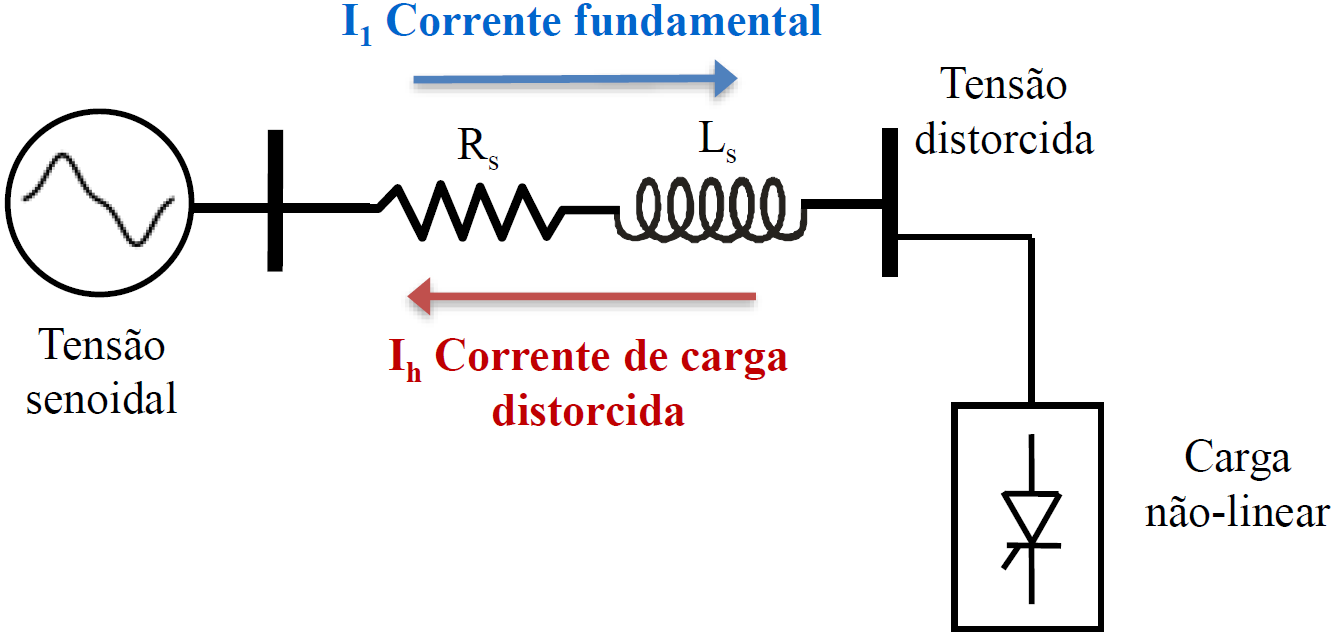
\includegraphics[width=12.5cm]{harmonicos}
\caption{Figura ilustrativa de harmônicos na rede \cite{PH}.}
\label{intro:fig1}
\end{figure}

\begin{figure}[H]
\hspace{0.4cm}
\centering
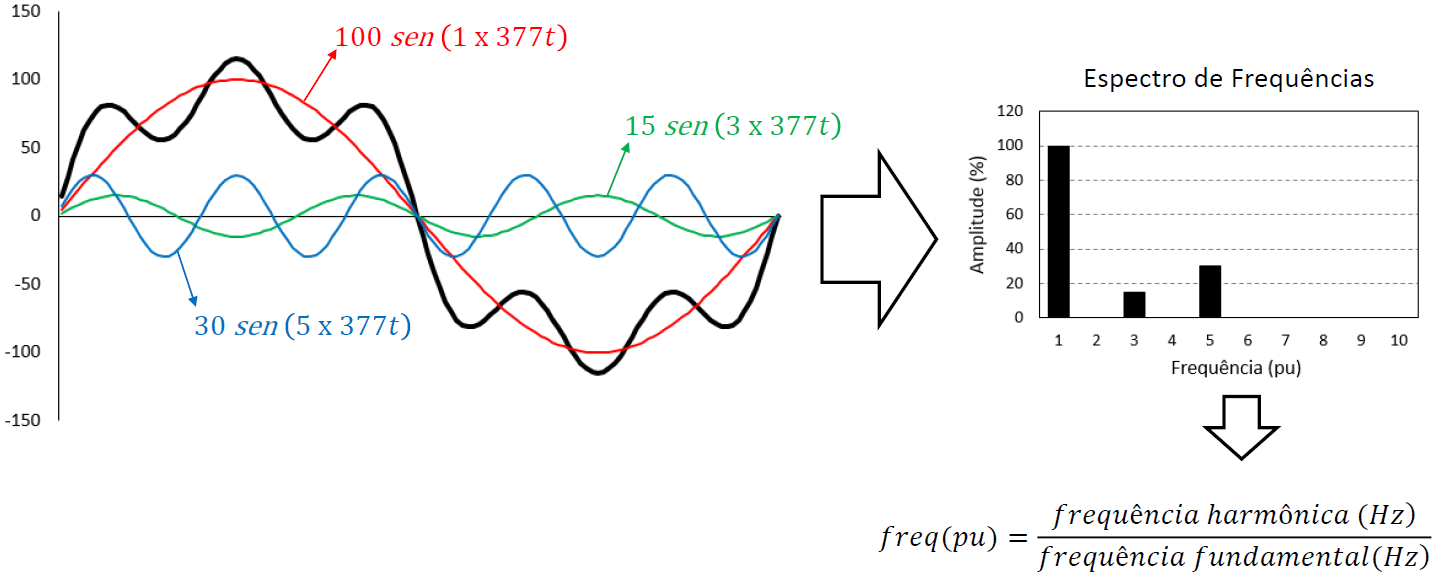
\includegraphics[width=12.5cm]{espectro}
\caption{Descrição em série de Fourier  e análise espectro de frequências \cite{PH}.}
\label{intro:fig2}
\end{figure}
\vspace{0.3cm}

\section{Preparação}
\subsection{Materiais e ferramentas} % 2,5%
\begin{enumerate}[1 -]
\item \emph{\textbf{Fonte:}}
Alimentará todo o circuito. Possui frequência de $60\ Hz$.

\item \emph{\textbf{Regulador de tensão (Varivolt):}}
Também chamado de autotransformador, permitirá obter o valor desejado de corrente a partir da regulagem correta da tensão fornecida pela fonte.

\item \emph{\textbf{Conectores:}}
Para as conexões no circuito foi utilizado majoritariamente cabos banana-banana.

\item \emph{\textbf{Medidor eletrônico KRON Mult K:}}
Possibilita encontrar a medição da potência real (P) - vatímetro, reativa (Q) e aparente (S) do circuito. Ele também possui função de cofasímetro, instrumento elétrico que mede o fator de potência (fp, $cos\theta$) ou o ângulo da impedância $\theta$ do circuito, para um circuito com a impedância $Z = Z\angle \theta$.

\item \emph{\textbf{Lâmpadas:}}
Foram utilizadas lâmpadas LED e incandescente, para investigar o carácter não linear dessas cargas e seu efeuto na rede.

\item \emph{\textbf{Reostato:}}
Carga resistiva para evitar dano na lâmpada LED. Foi setado para $10 \Omega$.

\item \emph{\textbf{Reator:}}
Para a segunda montagem utilizou-se um indutor na carga de $166$ mH.

\end{enumerate}


\subsection{Montagem} % 2,5%

\subsubsection{Lâmpadas (Cargas não lineares)}
A montagem realizada observa-se na Figura \ref{m1:esquema}, na qual são empregados medidores de tensão e de corrente digitais (\emph{Kron Mult-K Série 2}). A configuração usada no medidor \emph{Kron} foi TL = 0000 ($3\phi$ com Neutro - Carga Desequilibrada) e valor para a resistência medida foi de $R=10.1\Omega$ e foi aplicada uma tensão de fase $V_F=V_{AN}$ que variou de 10 a 100V. Lembrando que as lâmpadas a LED ou fluorescente compacta normalmente acendem após certo valor de tensão.

\vspace{1.5cm}
\begin{figure}[H]
\centering
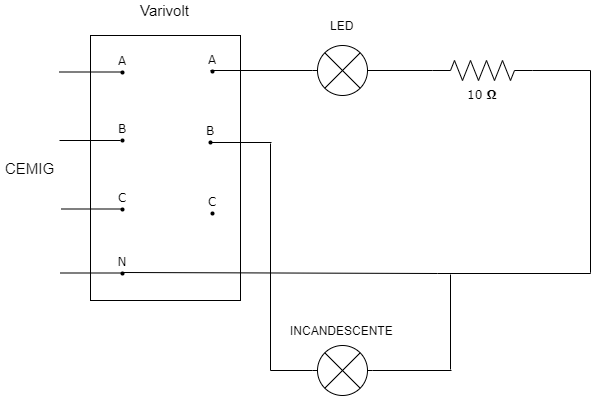
\includegraphics[width=13cm]{m1-circuito}
\caption{Montagem realizada para verificação de espectro para cargas não-lineares.}
\label{m1:esquema}
\end{figure}

\newpage
\subsubsection{Medições em ambiente com $f\ne 60Hz$}
Como na Figura \ref{m2:esquema}, nessa etapa é utilizado um retificador de onda completa para representar uma onda não-senoidal. O intuito dessa montagem é medir as grandezas de tensão e corrente nos terminais da carga utilizando-se de distintos medidores, inclusive não True RMS, para assim intuir a importância da utilização de equipamento de medição True RMS.

\vspace{1.5cm}
\begin{figure}[H]
\centering
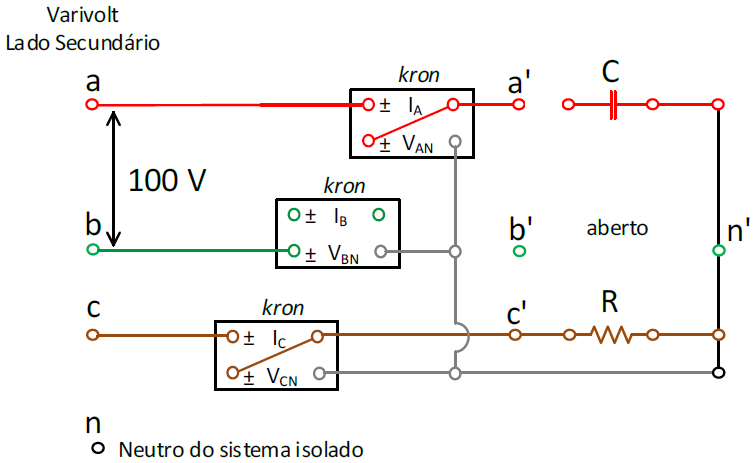
\includegraphics[width=13.3cm]{m2-circuito}
\caption{Montagem para experimento de ambiente com $f\ne 60Hz$.}
\label{m2:esquema}
\end{figure}
\vspace{0.1cm}


\newpage
\section{Dados Experimentais} \label{dados}

\subsubsection{Lâmpadas (Cargas não lineares)}
Do experimento para análise de tensão e corrente em cargas não lineares tem-se do dados comtemplados na Tabela \ref{m1:dados:kron} obtidos com o medidor \emph{Kron}. Já na Tabela \ref{m1:dados:truerms} estão os valores de tensão obtidos com o multímetro True RMS.

\vspace{0.8cm}
\begin{table}[H]
\centering \def\arraystretch{1.28}
\caption{Dados experimentais para o experimento com lâmpadas como carga.}
\label{m1:dados:kron}
\resizebox{\textwidth}{!}{%
\begin{tabular}{|c|c|c|c|c|c|c|c|c|c|}
\hline
$V_{F}$ (V) & Fase & $V_{F}$ (V) & $I_{L}$ & P (W) & Q (VAr) & S (VA) & FP & DTT (\%) & DTI (\%) \\ \hline
\multirow{2}{*}{10,0} & A & 10,47 & 0 & 0 & 0 & 0 & 0 & 4,73 & 0 \\ \cline{2-10} 
 & B & 10,67 & 0,112 & 1,182 & 1,156 & 1,194 & 0,991 & 4,09 & 9,08 \\ \hline
\multirow{2}{*}{20,0} & A &20,35 & 0 & 0 & 0 & 0 & 0 & 3,36 & 0\\ \cline{2-10} 
 & B & 20,86 & 0,14 & 2,907 & 0,287 & 2,92 & 0,995 & 3,36 & 6,51 \\ \hline
\multirow{2}{*}{30,0} & A & 30,84 & 0 & 0 & 0 & 0 & 0 & 2,97 & 0\\ \cline{2-10} 
 & B & 31,14 & 0,164 & 5,09 & 0,422 & 5,118 & 0,996 & 2,52 & 5,94 \\ \hline
\multirow{2}{*}{40,0} & A & 40,06 & 0 & 0 & 0 & 0 & 0 & 2,85 & 0 \\ \cline{2-10} 
 & B & 40.64 & 0,181 & 7,388 & 0,555 & 7,426 & 0,997 & 2,63 & 5,05\\ \hline
\multirow{2}{*}{50,0} & A &  50,02 & 0,127 & 5,037 & 3,862 & 6,338 & 0,792 & 2,820 & 31,29 \\ \cline{2-10} 
 & B & 50,15 & 0,203 & 10,15 & 0,715 & 10,19 & 0,998 & 2,58 & 4,390\\ \hline
\multirow{2}{*}{60,0} & A &  60,01 & 0,135 & 5,99 & 5,436 & 8,086 & 0,744 & 2,56 & 39,20\\ \cline{2-10} 
 & B & 60,32 & 0,223 & 13,45 & 0,853 & 13,45 & 0,998 & 2,59 & 4,340 \\ \hline
\multirow{2}{*}{70,0} & A & 70,12 & 0,143 & 7,097 & 7,069 & 10,03 & 0,704 & 2,7 & 46,75\\ \cline{2-10} 
 & B & 70,09 & 0,241 & 16,88 & 1,030 & 16,93 & 0,998 & 2,62 & 3,46 \\ \hline
\multirow{2}{*}{80,0} & A &  80,23 & 0,148 & 8,048 & 8,603 & 11,75 & 0,680 & 2,74 & 53,49 \\ \cline{2-10} 
 & B &  79,82 & 0,258 & 20,60 & 1,202 & 20,77 & 0,998 & 2,53 & 3,370\\ \hline
\multirow{2}{*}{90,0} & A & 90,32 & 0,144 & 8,764 & 9,454 & 12,79 & 0,679 & 2,51 & 60,16\\ \cline{2-10} 
 & B &  89,80 & 0,275 & 24,67 & 1,374 & 24,65 & 0,998 & 2,5 & 3,17 \\ \hline
\multirow{2}{*}{100,0} & A &  100,0 & 0,141 & 9,478 & 10,22 & 13,81 & 0,680 & 2,67 & 66,94 \\ \cline{2-10} 
 & B & 100,1 & 0,291 & 29,21 & 1,540 & 29,14 & 0,999 & 2,33 & 2,92\\ \hline
\end{tabular}%
}
\end{table}
\vspace{0.3cm}

\begin{table}[H]
\centering \small \def\arraystretch{1.28}
\caption{Tensões True RMS para a fase A (LED) e fase B (Incandescente)}
\label{m1:dados:truerms}
\begin{tabular}{c|c|c|}
\cline{2-3}
 & $V_A$ (V) & $V_B$ (V) \\ \hline
\multicolumn{1}{|c|}{10V} & 10,49 & 10,62 \\ \hline
\multicolumn{1}{|c|}{20V} & 20,59 & 20,99 \\ \hline
\multicolumn{1}{|c|}{30V} & 31,13 & 30,80 \\ \hline
\multicolumn{1}{|c|}{40V} & 40,60 & 40,47 \\ \hline
\multicolumn{1}{|c|}{50V} & 49,62 & 51,00 \\ \hline
\multicolumn{1}{|c|}{60V} & 60,4 & 61,9 \\ \hline
\multicolumn{1}{|c|}{70V} & 69,5 & 71,1 \\ \hline
\multicolumn{1}{|c|}{80V} & 80,3 & 81,7 \\ \hline
\multicolumn{1}{|c|}{90V} & 90,65 & 90,99 \\ \hline
\multicolumn{1}{|c|}{100V} & 100,0 & 101,2 \\ \hline
\end{tabular}
\end{table}
\vspace{0.4cm}

\subsubsection{Medições em ambiente com $f\ne 60Hz$}
Da montagem da Figura \ref{m2:esquema} pode-se retirar dados com o osciloscópio, tanto de imagem conforme a Figura \ref{m2:imagem}, quanto de CSV, no qual são discretizados os dados de tensão obtidos numa determinada frequência de amostragem $F_S$. Como o arquivo CSV obtido é demasiadamente extenso não será mostrado aqui. 

\vspace{1cm}
\begin{figure}[H]
\centering
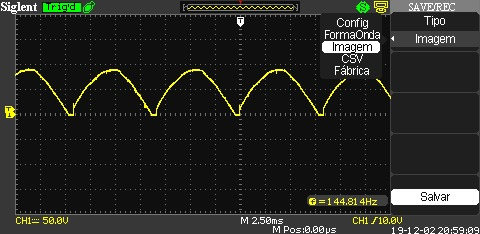
\includegraphics[width=13cm]{osc001}
\caption{Dado de imagem retirado do osciloscópio.}
\label{m2:imagem}
\end{figure}
\vspace{0.1cm}
 

\section{Análise sobre segurança} % 2,5%
Os óculos de segurança são Equipamentos de Proteção Individual (EPIs) e são utilizados para a proteção da área ao redor dos olhos contra qualquer tipo de detrito estranho, que possa causar irritação ou ferimentos. Também protegem contra faíscas, respingos de produtos químicos, detritos, poeira, radiação e etc \cite{safe}.
É importante a utilização desse equipamento durante os experimentos a fim de evitar qualquer dano, além de preparar o profissional para o manejo correto e seguro de qualquer equipamento.
Além disso, foi de extrema importância a presença do professor ou técnico na verificação da montagem do circuito antes de energizá-lo. Assim, reduziu-se riscos de curtos-circuitos ou sobrecarga na rede.

\vspace{0.2cm}
\section{Análise e discussão} % (quando houver) (70%)
\subsubsection{Descrição da corrente sobre as lâmpadas em série Fourier}
% - Obtenha, analiticamente, a série de Fourier da corrente que alimenta as lâmpadas.

\subsubsection{Comparação do valor RMS obtido com o experimental}
% - Com o resultado do item anterior, calcule o valor eficaz e compare com a indicação dos amperímetros.

\subsubsection{Espectro harmônico da corrente}
% - Usando alguma rotina computacional, obtenha o espectro harmônico da corrente e
% compare o resultado obtido com o item (a). Se necessário, aplique um filtro para
% frequências acima de 720 Hz. Neste caso, qual é a ordem harmônica de interesse neste
% relatório?

\subsubsection{Sobre a Distorção Harmônica Total (DHT)}
% - Pesquise sobre DHT, sua relação com essa aula e possíveis problemas causados em um
% circuito elétrico. Qual é o valor máximo admissível em uma instalação elétrica?



\vspace{1cm}
\section{Simulação computacional} % (10%);

\vspace{2cm}
\section{Conclusões} % (no mínimo 10 linhas) (5%);
Equipamentos não lineares são bastante comuns na rede, e interferem por meio do aparecimento de harmônicos na rede.

\newpage
\begin{thebibliography}{9} 
% Introdução
\bibitem{PH}
    P. H. O. Rezende,
    "Ondas Não Senoidais", 2018.

\bibitem{safe}
    SafetyTrabi,
    “Óculos de segurança: Saiba quando utilizar este EPI”, SafetyTrab, 2019.
 Disponível em:
 \url{https://www.safetytrab.com.br/blog/oculos-de-seguranca/}. Acesso em: ago. 2019.

\end{thebibliography}
\end{document}
